\documentclass{standalone}
\usepackage[dvipsnames]{xcolor}

\usepackage{tikz}
\usetikzlibrary{arrows.meta,shapes.geometric,positioning,matrix,calc,fit,decorations.pathreplacing}

\colorlet{States}{Melon!50}
\colorlet{Energies}{SkyBlue!50}
\colorlet{Rect}{Orchid!30}
\colorlet{Decision}{GreenYellow!30}
\colorlet{Frame1}{Magenta}
\colorlet{Frame2}{NavyBlue}

\begin{document}
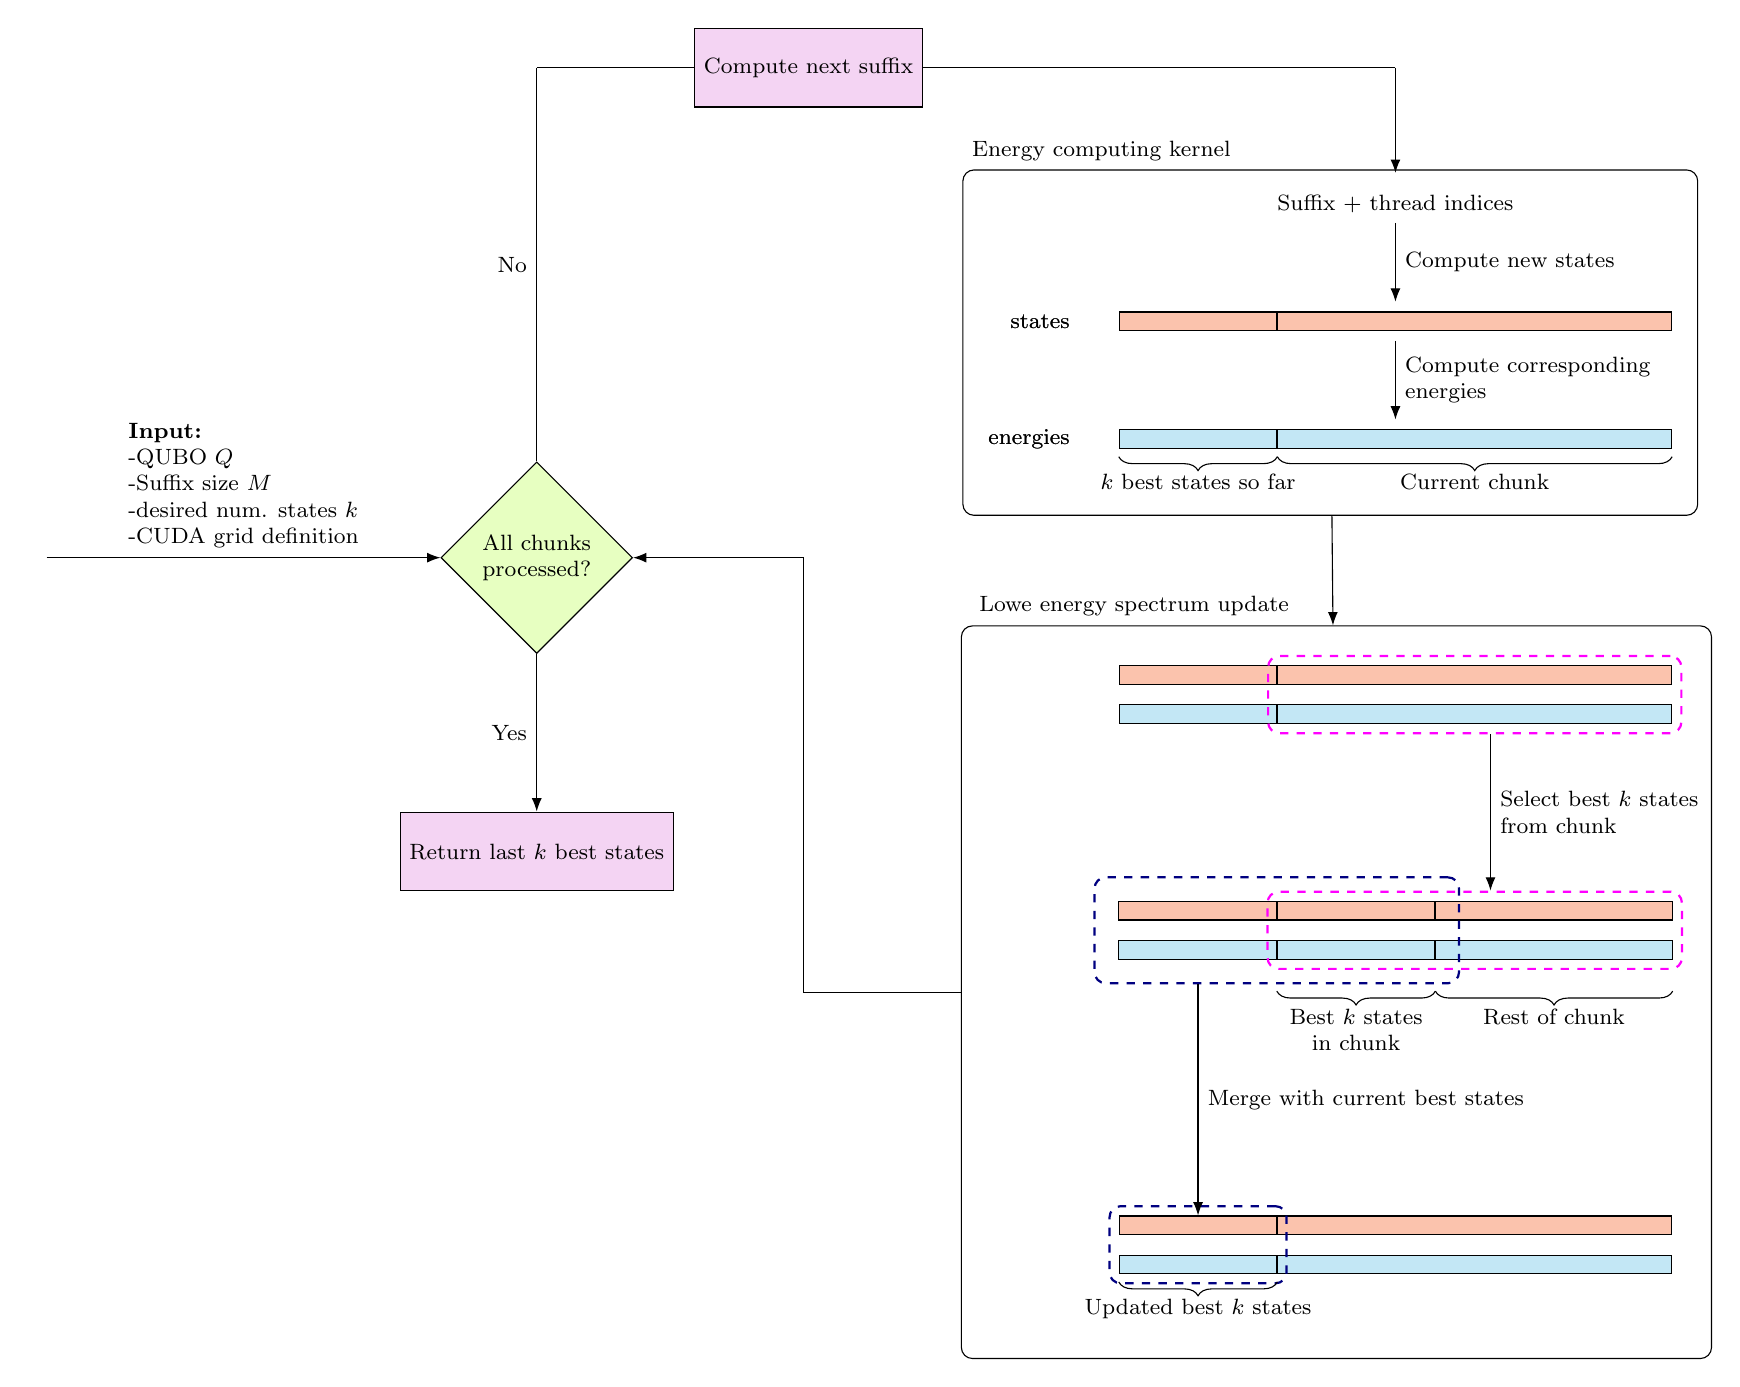
\begin{tikzpicture}[
    memcell/.style={draw, rectangle, minimum width=0.2cm, minimum height=0.2cm},
    memarray/.style={matrix of nodes, nodes in empty cells, column 1/.style={nodes={minimum width=2cm}}},
    states/.style={memarray, nodes={memcell, fill=States}},
    energies/.style={memarray, nodes={memcell, fill=Energies}},
    rect/.style={minimum height=1cm, fill=Rect, draw, rectangle},
    decision/.style={draw, align=center, diamond, fill=Decision},
    every node/.style={font={\footnotesize}},
    brace/.style={decorate,decoration={brace,amplitude=5pt,mirror,raise=1mm}},
    brace2/.style={decorate,decoration={brace,amplitude=5pt,mirror,raise=4mm}},
    subroutine/.style={draw, rounded corners},
    subsubroutine/.style={subroutine,dashed,thick}
  ]
  \node (start) {};
  \node[decision, right=5cm of start] (decision) {All chunks\\processed?};
  \coordinate [above=5cm of decision] (c1);
  \node[rect, right=2cm of c1] (suffix) {Compute next suffix};
  \coordinate [right=6cm of suffix] (c2);

  \node [below=1.5cm of c2] (kernelinput) {Suffix + thread indices};

  \matrix [states, column 2/.style={nodes={minimum width=5cm}}, below=1cm of kernelinput]
  (states1)
  {
     & \\
  };
  \node [left=0.5cm of states1-1-1] {states};

  \matrix [energies, column 2/.style={nodes={minimum width=5cm}}, below=1cm of states1]
  (energies1)
  {
     & \\
  };
  \node [left=0.5cm of energies1-1-1] (energies1label) {energies};

  \draw
  [brace]
  (energies1-1-2.south west)
  --
  (energies1-1-2.south east)
  node [midway, below=2mm] {\footnotesize Current chunk};

  \draw [brace]
  (energies1-1-1.south west)
  --
  (energies1-1-1.south east)
  node [midway, below=2mm,align=center] (brace1)
  {\footnotesize $k$ best states \footnotesize so far};

  \node [
  fit=(energies1label) (states1) (brace1) (kernelinput),
  subroutine,
  inner sep=2mm,
  label={[anchor=south west]155:{{Energy computing kernel}}}
  ]
  (kernel) {};

  \matrix [states, column 2/.style={nodes={minimum width=5cm}}, below=2.5cm of energies1]
  (states2)
  {
     & \\
  };
  \node [left=0.5cm of states1-1-1] {states};

  \matrix [energies, column 2/.style={nodes={minimum width=5cm}}, below=0cm of states2]
  (energies2)
  {
     & \\
  };
  \node [left=0.5cm of energies1-1-1] (energies1label) {energies};

  \node[fit=(energies2-1-2) (states2-1-2),subsubroutine,draw=Frame1] (selectk) {};

  \matrix [
    states,
    column 2/.style={nodes={minimum width=2cm}},
    column 3/.style={nodes={minimum width=3cm}},
    below=2cm of energies2
  ]
  (states3)
  {
     &  & \\
  };

  \matrix [
    energies,
    column 2/.style={nodes={minimum width=2cm}},
    column 3/.style={nodes={minimum width=3cm}},
    below=0cm of states3,
  ]
  (energies3)
  {
     &  & \\
  };

  \draw [brace2]
  (energies3-1-2.south west)
  --
  (energies3-1-2.south east)
  node [midway, below=5mm, align=center] {Best $k$ states\\in chunk};

  \draw [brace2]
  (energies3-1-3.south west)
  --
  (energies3-1-3.south east)
  node [midway, below=5mm,align=center] (brace1) {\footnotesize Rest of chunk};

  \node[fit=(energies3-1-2) (states3-1-3), subsubroutine, draw=Frame1] (selectedk) {};
  \node[fit=(energies3-1-2) (states3-1-1), subsubroutine, draw=Frame2, inner sep=3mm] (premerge) {};

  \matrix [
    states,
    column 2/.style={nodes={minimum width=5cm}},
    below=3cm of energies3
  ]
  (states4)
  {
     & \\
  };
  \node [left=0.5cm of states4-1-1,opacity=0] (stateslabel) {states};

  \matrix [
    energies,
    column 2/.style={nodes={minimum width=5cm}},
    below=0cm of states4
  ]
  (energies4)
  {
     & \\
  };

  \node[fit=(energies4-1-1) (states4-1-1), subsubroutine, draw=Frame2] (postmerge) {};

  \node[opacity=0, below=2mm of energies4] (phony) {};
  \draw [brace]
  (energies4-1-1.south west)
  --
  (energies4-1-1.south east)
  node [midway, below=2mm,align=center] (brace1) {Updated best $k$ states};

  \node[
  fit=(states2-1-1) (energies4-1-2) (phony) (stateslabel),
  subroutine,
  inner sep=5mm,
  label={[anchor=south west] above left:{{Lowe energy spectrum update}}}
  ]
  (mergesubroutine) {};

  \coordinate[left=2cm of mergesubroutine] (c4);

  \node[below=2cm of decision,rect,rectangle,draw] (return) {Return last $k$ best states};
  \draw[-Latex] (start) -- (decision) node[midway, above, align=left] {\textbf{Input:}\\-QUBO $Q$\\-Suffix size $M$\\-desired num. states $k$\\-CUDA grid definition};
  \draw (decision) -- (c1) node[left,midway] {No};
  \draw (c1) -- (suffix);
  \draw (suffix) -- (c2);
  \draw[-Latex] (kernelinput) -- (states1) node[midway, right] {Compute new states};
  \draw[-Latex] (states1) -- (energies1) node[midway, right, align=left] {Compute corresponding\\energies};
  \draw[-Latex] (kernel) -- (mergesubroutine);
  \draw[-Latex] (c2) -- ($(kernelinput)+(0,0.4cm)$);

  \draw[-Latex]
  ($(selectk.south)+(0.2cm,0)$)
  --
  ($(selectedk.north)+(0.2cm,0)$)
  node[midway,right,align=left] {Select best $k$ states\\from chunk};

  \draw[-Latex]
  ($(premerge.south east)!(states4-1-1.north)!(premerge.south west)$)
  --
  (states4-1-1)
  node[midway,right] {Merge with current best states};

  \draw (mergesubroutine) -- (c4);
  \draw[-Latex] (c4) |- (decision.east);
  \draw[-Latex] (decision) -- (return) node[midway,left] {Yes};
\end{tikzpicture}
\end{document}
